\chapter{Análise da influência}
\label{ch:mineracao}

Após as representações haverem sido mensuradas, chegamos no objetivo de todo o
processo: a análise da influência. Como já foi descrito em seções anteriores, o
entendimento da dinâmica da influência na rede pode facilitar a criação de
campanhas publicitárias virais baseadas no boca-a-boca; a difusão de novas
informações para a comunidade; comunicação interna corporativa; reconhecimento de
especialistas e atores chaves na organização; otimizar buscas
\citep{Kirchhoff2009}. Abordagens recentes focam em modelos probabilísticos e
comportamentais para estimar a dinâmica da influência. Métodos mais tradicionais
de redes sociais voltaram-se para métricas individuais de proeminência para
reconhecer atores chave. Em \citet{Kempe2003} encontramos uma comparação
mostrando que apesar de encontrar um subconjunto ótimo de $n$ atores tal que
maximize a dispersão da influência seja um problema $NP$, algoritmos que
aproximam a solução para modelos dinâmicos superam soluções baseadas na simples
escolha de atores centrais em 18\% (para a métrica de grau) e 40\% (para a
métrica de proximidade). Porém, essas métricas são consideradas na literatura
como sendo de pouca expressividade, o que torna a comparação de
\citeauthor{Kempe2003} inconclusiva. Outras métricas melhores fundamentadas
poderiam obter um resultado melhor, dessa forma, permitindo que a análise
tradicional de redes sociais seja uma alternativa na análise de influência.

\section{Sobre Proeminência}
\label{sec:sobre-proem}
Proeminência é a característica dos relacionamentos de um ator que o põe em
evidência para outros atores na rede \citep{Wasserman}. A proeminência,
academicamente, foi separada em dois aspectos: centralidade e prestígio.
Centralidade é como o ator se posiciona na rede, sua interação e envolvimento com
os outros. Prestígio é como os outros atores se posicionam em relação a ele, como
interagem e envolvem-se com ele \citep{Knoke1983}.

Nosso objetivo, identificar atores chaves para processos de influência da rede,
está relacionado diretamente com o conceito de proeminência de forma que podemos
dizer que a usaremos como uma aproximação da influência do ator na transmissão de
conhecimento, inovações e opiniões pela rede. Por estes motivos, cuidado especial
deve ser tomado sobre a forma como calcularemos a proeminência e que
características são esperadas da representação da rede mensurada.

Durante décadas pesquisadores de redes sociais se debruçaram sobre o estudo da
proeminência, desenvolvendo inúmeras métricas que conjuntamente são chamadas de
métricas de centralidade. Quando calculadas considerando os caminhos que
\textbf{saem} do ator, referem-se a sua centralidade propriamente dita. Quando
considera-se os caminhos que \textbf{chegam} no ator, referem-se ao seu
prestígio. Não obstante tenha o comum senso de que essas métricas referem-se de
alguma forma à proeminência do ator, a forma específica tem ficado a cargo de
cada pesquisador que já atribuiu ao seu resultado interpretações como autonomia,
controle, risco, influência, corretagem (\emph{brokerage}), independência,
etc.

\citet{Freeman1979} revisou as métricas existentes à época e as compilou em três
principais centralidades: por grau, por proximidade (\emph{closeness}) e por
intermediação (\emph{betweenness}). Interpretando seus resultados em relação a
quanto o grafo se aproxima de uma estrutura de estrela (\figref{fig:star}),
sua visão de centralização ideal, onde suas métricas alcançam o máximo.

\begin{figure}[h!]
  \centering
    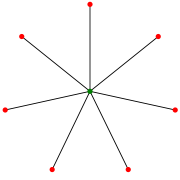
\includegraphics[width=0.3\textwidth]{imgs/star.png}
    \caption{Gráfico estrela}
  	\label{fig:star}
\end{figure}

Recentemente, \citet{Borgatti2006} nos ofereceram uma outra reposta para a
questão: O que as métricas de centralidade medem? E chegaram a conclusão que
todas elas investigam o relacionamento do nó com os possíveis caminhos do grafo.
Em sua tipologia para a classificação das métricas de centralidade, propõem
quatro dimensões: tipo do caminho, propriedade do caminho, tipo do envolvimento e
forma de agregação. Em outras palavras, toda métrica de centralidade é uma forma
de agregar uma propriedade dos caminhos de determinado tipo em que o nó tem um
determinado envolvimento. Das quatro dimensões, duas são de maior importância:
propriedade do caminho e tipo de envolvimento.

\subsection{Tipo de envolvimento} 

O tipo de envolvimento é a dimensão de classificação proposta por Borgatti que
se traduz na maior variância nos resultados. Pode ser de dois tipos: radial ou
medial.

Métricas radiais são as que analisam os caminhos em que o nó está numa das
pontas, ou seja, que saem ou chegam nele. Exemplos de métricas radiais são as
centralidades de grau e proximidade de Freeman. A análise de Borgatti et al veio
confirmar o que as evidências empíricas já sugeriam, que as métricas radiais
representam a parcela de responsabilidade que o nó tem na coesão total da rede e
que, por este motivo, se enfraquecem a medida que a rede não se adequa ao padrão
de núcleo-periferia \citep{Nakao1990}.

Já as ditas mediais analisam os caminhos que passam pelo nó, classificando-o em
seu papel de \emph{gateway} entre partes da rede. O \emph{betweenness} de
Freeman é um exemplo de métrica medial. São mais estáveis em relação à
característica de núcleo-periferia, por outro lado tendem a dar maior importância
a atores que conectam grupos distintos, mas que se encontram na periferia dos
mesmos.

Os dois tipos são complementares e mais de uma métrica devem ser combinadas
(\citealt{Stephenson1989}; apud \citealt{Wasserman}). Pelo fato de que usaremos
métricas radiais de centralidade para estimar a influência do ator na rede, daí
concluímos que quanto mais próximo a representação estiver do modelo de
\textbf{núcleo-periferia}, melhor será a aplicabilidade das métricas radiais de
centralidade.

\subsection{Propriedade do caminho}

Borgatti define dois tipos de propriedade: distância e volume. A
propriedade do tipo distância mais comum é a geodésica que é a quantidade de
arcos presentes no menor caminho entre um ator e outro. Volume refere-se à
quantidade de caminhos entre os nós. As centralidades por grau e
\emph{betweenness} são exemplos de métricas que usam o volume dos caminhos,
enquanto que \emph{closeness} usa distância.

O critério de escolha depende da aplicação. Para o nosso caso, queremos modelar o
efeito da influência entre os pares na transmissão de informação. Nesse sentido,
quanto mais atores próximos estiverem tentando convencer alguém de algo, maior
será sua influência sobre este \citep{Watts2007}. Daí temos, naturalmente, a
preferência sobre métricas relacionadas a volume, no lugar de distância, já que
representa diretamente a quantidade de caminhos que existem entre os nós.

\subsection{Redundância na proeminência}

Vimos no \secref{sec:criterios} como calcular a redundância das conexões entre
representações disponíveis, porém também é interessante observar a relação que há
entre os resultados da análise de cada rede. Para esse fim utilizaremos também a
correlação linear de Pearson entre os vetores de proeminência calculado de forma
que duas redes podem estar positivamente relacionadas, aparentemente
independentes ou negativamente relacionadas. Um critério baseado na proeminência
pode correlacionar redes estruturalmente bastante diferentes, mas que resultam no
sobressaimento dos mesmos atores em termos de importância. Porém, se o objetivo
for minizar a redundância do ponto de vista da ordenação final dos atores por
grau de proeminência para a utilização em outros algoritmos como por exemplo,
escolha de subconjunto ótimo para marketing viral, então talvez este critério
seja o mais apropriado.

\subsection{Relevância na proeminência}
\label{sec:rel_proe}

Quando tudo o que temos é a rede, para medirmos proeminência dos atores
precisamos ser capazes também de medir sua aplicabilidade. Vimos que para alguns
tipos de métricas a rede precisa aprensetar determinado padrão de aglomeração.
Por esta razão, podemos saber \emph{a priori} quando uma representação vai
produzir métricas significativas de proeminência. É sabido que redes sociais são
formadas por diversas comunidades sobrepostas \citep{Palla2005} e por isso uma
representação com alto grau de núcleo/periferia nessas condições é pouco
provável. Uma abordagem seria quebrar a rede em suas comunidades para a partir
daí encontrar os atores centrais de cada uma, existem diversas ferramentas de
decomposição da rede em \emph{k-cliques}, \emph{k-plexes}, \emph{k-cores} para
grafos valorados e direcionados (\citealt{Peay1975, Doreian1969, Freeman1992};
apud \citealt{Wasserman}), mas todas elas tendem a ignorar atores pendentes que
compõem grande parte da periferia.

Um modelo mais interessante para o nosso problema é a chamada comunidade de
prática. A teoria das comunidades de prática não nasceu no meio sociométrico e é
voltada ao estudo da gestão do conhecimento, porém o trabalho de
\citet{Schenkel2002} revisa as características estruturais típicas das
comunidades de prática e sugere quatro delas muito similares ao que estamos
procurando:

\begin{description}
\item[Conectada] A rede possui apenas um componente;
\item[Densa] A média das conexões por ator é alta; o que é considerado
alto varia a depender do tamanho da rede e, por tanto, da periferia;
\item[Compacto] A distância média entre os atores é menor do que o comum para
\emph{small-worlds}, cujo crescimento é logarítmico em relação ao crescimento
da rede;
\item[Núcleo/Periferia] A rede exibe um padrão de núcleo periferia, isto é, alto
grau de \emph{scale-freeness}.
\end{description}

Resta-nos encontrar maneiras de reconhecer essas comunidades e, mais importante,
quais atores a compõem. Comunidades de prática foram definidas como: um grupo de
pessoas informalmente e contextualmente conectadas a uma situação de trabalho em
que estão empregando uma competência comum na perseguição de um objetivo comum
\citep{Wenger1999}. Essas situações de trabalho, no entanto, podem ser
generalizadas para situações que envolvem perícia, conhecimento técnico e por
isso encontraremos comunidades de práticas não apenas no contexto organizacional,
mas entre hobbistas também. O conhecimento em tais comunidades é compartilhado
através de narrativas, conversação, \emph{mentoring} e aprendizagem por
experimentos \citep{Brown1991, Lave1991a}, tais atividades podem ser
transferidas para o meio digital \citep{Hildreth1998, Kimble2001} e deixam
rastros que podem ser mensurados para reconstruir a rede
\citep{Tyler2005, Welser2007}.

É de se esperar, por tanto, que os membros de comunidades de prática se reunam
em torno de focos de interação ondem possam compartilhar histórias, como por
exemplo comunidades virtuais. Para diminuir o ambiguidade do termo, utilizaremos
a palavra \emph{coletividade} quando nos referirmos à comunidade virtual na
qual os atores se afiliam digitalmente. Podemos construir uma rede
de coletividades, onde um nó está ligado a outro se possuem membros em comum,
essa rede é menos sucetível à existência de pendentes e por isso podemos aplicar
algoritmos como os descritos em \citet{Palla2005} para reconhecer coletividades
que se aglomeram em grupos. Essas coletividades poderiam ser usadas depois para
filtrar a rede de atores e verificar se atendem às características de
comunidades de prática, aumentando a relevância da representação para a análise
da influência.

Outra possibilidade é tentar identificar o objetivo ou competência comum que
reúne a comunidade através de mineração de texto. Possibilidades vão desde
encontrar a distância relativa entre os atores baseados em quais palavras
aparecem em seus textos \citep{Reichling2005}, até criar uma ontologia dos termos
propriamente dita e a partir daí estimar uma conexão entre os atores
\citep{Mori2006}. \citet{Spertus2005} propõem o uso da métrica de similaridade
para termos extraídos do texto TF-IDF \citep{Salton1989, Frakes1992} e em
\citet{MATSUO2007} encontramos uma versão aperfeiçoada que diminui a necessidade
de um \emph{corpus} da linguagem. A similaridade, dessa forma, pode indicar uma
homofilia de interesses quando cruzada com as representações mensuradas das
interações, essa homofilia poderia ser usada então para filtrar a rede de atores
e, em verificando as características de comunidades de prática, também vir a
aumentar a relevância da representação na análise da influência.